\documentclass[12pt,a4paper]{article}
        \usepackage{graphicx}
        \usepackage{geometry}
        \geometry{margin=2cm}
        \usepackage{helvet}
        \usepackage{xcolor}
        \usepackage{amsmath} % for bmatrix
        \setlength{\parindent}{0pt}  % No indentation globally
        \renewcommand{\familydefault}{\sfdefault}
        \usepackage[german]{babel}% for glqq / grqq

        \begin{document}\begin{center}
                \Huge \textbf{Benzene} \\[1cm]
                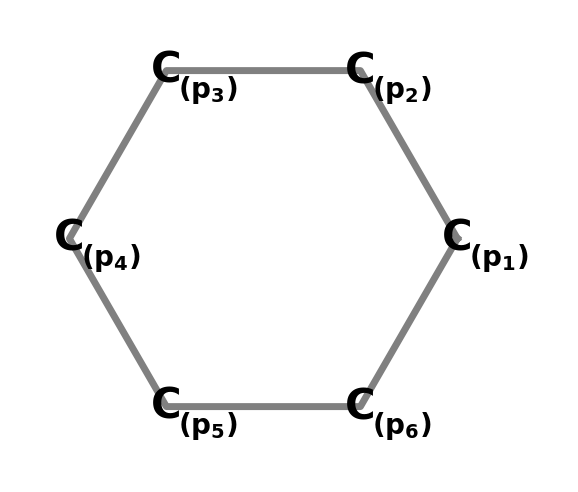
\includegraphics[width=0.5\textwidth]{benzene} \\[0.5cm]
                \Large Point Group: \textbf{D6h}
            \end{center}\newpage\section*{p orbitals}
Symmetry behavior of the p-orbitals:
$$\mathsf{\Gamma}_{red} = \,6 E\;; \,-2 C'2\;; \,-6 \sigma h\;; \,2 \sigma v\;$$
$$\mathsf{\Gamma}_{irred} = \,1 B2g\;\oplus{}\,1 E1g\;\oplus{}\,1 A2u\;\oplus{}\,1 E2u\;$$


\begin{itemize}
\item SALC of B2g: \quad $\frac{\sqrt{6} \left(\text{p}_{1} - \text{p}_{2} + \text{p}_{3} - \text{p}_{4} + \text{p}_{5} - \text{p}_{6}\right)}{6}$
\item SALC of E1g: \quad $\frac{\sqrt{3} \left(2 \text{p}_{1} + \text{p}_{2} - \text{p}_{3} - 2 \text{p}_{4} - \text{p}_{5} + \text{p}_{6}\right)}{6}$
\item SALC of E1g: \quad $\frac{\text{p}_{2}}{2} + \frac{\text{p}_{3}}{2} - \frac{\text{p}_{5}}{2} - \frac{\text{p}_{6}}{2}$
\item SALC of A2u: \quad $\frac{\sqrt{6} \left(\text{p}_{1} + \text{p}_{2} + \text{p}_{3} + \text{p}_{4} + \text{p}_{5} + \text{p}_{6}\right)}{6}$
\item SALC of E2u: \quad $\frac{\sqrt{3} \left(2 \text{p}_{1} - \text{p}_{2} - \text{p}_{3} + 2 \text{p}_{4} - \text{p}_{5} - \text{p}_{6}\right)}{6}$
\item SALC of E2u: \quad $\frac{\text{p}_{2}}{2} - \frac{\text{p}_{3}}{2} + \frac{\text{p}_{5}}{2} - \frac{\text{p}_{6}}{2}$
\end{itemize}
Put together these SALCs form the following Hamilton matrices:
     $$ H_{B2g}= \begin{pmatrix}\tilde{\alpha} - 2 \tilde{\beta}\end{pmatrix}$$ 
     $$ H_{E1g}= \begin{pmatrix}\tilde{\alpha} + \tilde{\beta} & 0\\0 & \tilde{\alpha} + \tilde{\beta}\end{pmatrix}$$ 
     $$ H_{A2u}= \begin{pmatrix}\tilde{\alpha} + 2 \tilde{\beta}\end{pmatrix}$$ 
     $$ H_{E2u}= \begin{pmatrix}\tilde{\alpha} - \tilde{\beta} & 0\\0 & \tilde{\alpha} - \tilde{\beta}\end{pmatrix}$$ 


Solving Hückels secular equations, that follow from these H, leads to:
\begin{itemize}
\item orbital of A2u with energy = 
                                $\tilde{\alpha} + 2 \tilde{\beta}$ \\
( 
$$
\begin{pmatrix}1\end{pmatrix} * \left(\begin{array}{c}\text{1. SALC in A2u}\end{array}\right) = \begin{pmatrix}1\end{pmatrix} * \begin{pmatrix}\frac{\sqrt{6} \text{p}_{1}}{6} + \frac{\sqrt{6} \text{p}_{2}}{6} + \frac{\sqrt{6} \text{p}_{3}}{6} + \frac{\sqrt{6} \text{p}_{4}}{6} + \frac{\sqrt{6} \text{p}_{5}}{6} + \frac{\sqrt{6} \text{p}_{6}}{6}\end{pmatrix} 
 $$ $$ = \frac{\sqrt{6} \left(\text{p}_{1} + \text{p}_{2} + \text{p}_{3} + \text{p}_{4} + \text{p}_{5} + \text{p}_{6}\right)}{6} 
 $$ 
 )

\item orbital of E1g with energy = 
                                $\tilde{\alpha} + \tilde{\beta}$ \\
( 
$$
\begin{pmatrix}1 & 0\end{pmatrix} * \left(\begin{array}{c}\text{1. SALC in E1g} \\ \text{2. SALC in E1g}\end{array}\right) = \begin{pmatrix}1 & 0\end{pmatrix} * \begin{pmatrix}\frac{\sqrt{3} \text{p}_{1}}{3} + \frac{\sqrt{3} \text{p}_{2}}{6} - \frac{\sqrt{3} \text{p}_{3}}{6} - \frac{\sqrt{3} \text{p}_{4}}{3} - \frac{\sqrt{3} \text{p}_{5}}{6} + \frac{\sqrt{3} \text{p}_{6}}{6}\\\frac{\text{p}_{2}}{2} + \frac{\text{p}_{3}}{2} - \frac{\text{p}_{5}}{2} - \frac{\text{p}_{6}}{2}\end{pmatrix} 
 $$ $$ = \frac{\sqrt{3} \left(2 \text{p}_{1} + \text{p}_{2} - \text{p}_{3} - 2 \text{p}_{4} - \text{p}_{5} + \text{p}_{6}\right)}{6} 
 $$ 
 )

\item orbital of E1g with energy = 
                                $\tilde{\alpha} + \tilde{\beta}$ \\
( 
$$
\begin{pmatrix}0 & 1\end{pmatrix} * \left(\begin{array}{c}\text{1. SALC in E1g} \\ \text{2. SALC in E1g}\end{array}\right) = \begin{pmatrix}0 & 1\end{pmatrix} * \begin{pmatrix}\frac{\sqrt{3} \text{p}_{1}}{3} + \frac{\sqrt{3} \text{p}_{2}}{6} - \frac{\sqrt{3} \text{p}_{3}}{6} - \frac{\sqrt{3} \text{p}_{4}}{3} - \frac{\sqrt{3} \text{p}_{5}}{6} + \frac{\sqrt{3} \text{p}_{6}}{6}\\\frac{\text{p}_{2}}{2} + \frac{\text{p}_{3}}{2} - \frac{\text{p}_{5}}{2} - \frac{\text{p}_{6}}{2}\end{pmatrix} 
 $$ $$ = \frac{\text{p}_{2}}{2} + \frac{\text{p}_{3}}{2} - \frac{\text{p}_{5}}{2} - \frac{\text{p}_{6}}{2} 
 $$ 
 )

\item orbital of E2u with energy = 
                                $\tilde{\alpha} - \tilde{\beta}$ \\
( 
$$
\begin{pmatrix}1 & 0\end{pmatrix} * \left(\begin{array}{c}\text{1. SALC in E2u} \\ \text{2. SALC in E2u}\end{array}\right) = \begin{pmatrix}1 & 0\end{pmatrix} * \begin{pmatrix}\frac{\sqrt{3} \text{p}_{1}}{3} - \frac{\sqrt{3} \text{p}_{2}}{6} - \frac{\sqrt{3} \text{p}_{3}}{6} + \frac{\sqrt{3} \text{p}_{4}}{3} - \frac{\sqrt{3} \text{p}_{5}}{6} - \frac{\sqrt{3} \text{p}_{6}}{6}\\\frac{\text{p}_{2}}{2} - \frac{\text{p}_{3}}{2} + \frac{\text{p}_{5}}{2} - \frac{\text{p}_{6}}{2}\end{pmatrix} 
 $$ $$ = \frac{\sqrt{3} \left(2 \text{p}_{1} - \text{p}_{2} - \text{p}_{3} + 2 \text{p}_{4} - \text{p}_{5} - \text{p}_{6}\right)}{6} 
 $$ 
 )

\item orbital of E2u with energy = 
                                $\tilde{\alpha} - \tilde{\beta}$ \\
( 
$$
\begin{pmatrix}0 & 1\end{pmatrix} * \left(\begin{array}{c}\text{1. SALC in E2u} \\ \text{2. SALC in E2u}\end{array}\right) = \begin{pmatrix}0 & 1\end{pmatrix} * \begin{pmatrix}\frac{\sqrt{3} \text{p}_{1}}{3} - \frac{\sqrt{3} \text{p}_{2}}{6} - \frac{\sqrt{3} \text{p}_{3}}{6} + \frac{\sqrt{3} \text{p}_{4}}{3} - \frac{\sqrt{3} \text{p}_{5}}{6} - \frac{\sqrt{3} \text{p}_{6}}{6}\\\frac{\text{p}_{2}}{2} - \frac{\text{p}_{3}}{2} + \frac{\text{p}_{5}}{2} - \frac{\text{p}_{6}}{2}\end{pmatrix} 
 $$ $$ = \frac{\text{p}_{2}}{2} - \frac{\text{p}_{3}}{2} + \frac{\text{p}_{5}}{2} - \frac{\text{p}_{6}}{2} 
 $$ 
 )

\item orbital of B2g with energy = 
                                $\tilde{\alpha} - 2 \tilde{\beta}$ \\
( 
$$
\begin{pmatrix}1\end{pmatrix} * \left(\begin{array}{c}\text{1. SALC in B2g}\end{array}\right) = \begin{pmatrix}1\end{pmatrix} * \begin{pmatrix}\frac{\sqrt{6} \text{p}_{1}}{6} - \frac{\sqrt{6} \text{p}_{2}}{6} + \frac{\sqrt{6} \text{p}_{3}}{6} - \frac{\sqrt{6} \text{p}_{4}}{6} + \frac{\sqrt{6} \text{p}_{5}}{6} - \frac{\sqrt{6} \text{p}_{6}}{6}\end{pmatrix} 
 $$ $$ = \frac{\sqrt{6} \left(\text{p}_{1} - \text{p}_{2} + \text{p}_{3} - \text{p}_{4} + \text{p}_{5} - \text{p}_{6}\right)}{6} 
 $$ 
 )

\end{itemize}



\newpage \section*{s orbitals}
Symmetry behavior of the s-orbitals:
$$\mathsf{\Gamma}_{red} = \,6 E\;; \,2 C'2\;; \,6 \sigma h\;; \,2 \sigma v\;$$
$$\mathsf{\Gamma}_{irred} = \,1 A1g\;\oplus{}\,1 E2g\;\oplus{}\,1 B1u\;\oplus{}\,1 E1u\;$$


\begin{itemize}
\item SALC of A1g: \quad $\frac{\sqrt{6} \left(\text{s}_{1} + \text{s}_{2} + \text{s}_{3} + \text{s}_{4} + \text{s}_{5} + \text{s}_{6}\right)}{6}$
\item SALC of E2g: \quad $\frac{\sqrt{3} \left(2 \text{s}_{1} - \text{s}_{2} - \text{s}_{3} + 2 \text{s}_{4} - \text{s}_{5} - \text{s}_{6}\right)}{6}$
\item SALC of E2g: \quad $\frac{\text{s}_{2}}{2} - \frac{\text{s}_{3}}{2} + \frac{\text{s}_{5}}{2} - \frac{\text{s}_{6}}{2}$
\item SALC of B1u: \quad $\frac{\sqrt{6} \left(\text{s}_{1} - \text{s}_{2} + \text{s}_{3} - \text{s}_{4} + \text{s}_{5} - \text{s}_{6}\right)}{6}$
\item SALC of E1u: \quad $\frac{\sqrt{3} \left(2 \text{s}_{1} + \text{s}_{2} - \text{s}_{3} - 2 \text{s}_{4} - \text{s}_{5} + \text{s}_{6}\right)}{6}$
\item SALC of E1u: \quad $\frac{\text{s}_{2}}{2} + \frac{\text{s}_{3}}{2} - \frac{\text{s}_{5}}{2} - \frac{\text{s}_{6}}{2}$
\end{itemize}
Put together these SALCs form the following Hamilton matrices:
     $$ H_{A1g}= \begin{pmatrix}\tilde{\alpha}_{s} + 2 \tilde{\beta}_{s}\end{pmatrix}$$ 
     $$ H_{E2g}= \begin{pmatrix}\tilde{\alpha}_{s} - \tilde{\beta}_{s} & 0\\0 & \tilde{\alpha}_{s} - \tilde{\beta}_{s}\end{pmatrix}$$ 
     $$ H_{B1u}= \begin{pmatrix}\tilde{\alpha}_{s} - 2 \tilde{\beta}_{s}\end{pmatrix}$$ 
     $$ H_{E1u}= \begin{pmatrix}\tilde{\alpha}_{s} + \tilde{\beta}_{s} & 0\\0 & \tilde{\alpha}_{s} + \tilde{\beta}_{s}\end{pmatrix}$$ 


Solving Hückels secular equations, that follow from these H, leads to:
\begin{itemize}
\item orbital of A1g with energy = 
                                $\tilde{\alpha}_{s} + 2 \tilde{\beta}_{s}$ \\
( 
$$
\begin{pmatrix}1\end{pmatrix} * \left(\begin{array}{c}\text{1. SALC in A1g}\end{array}\right) = \begin{pmatrix}1\end{pmatrix} * \begin{pmatrix}\frac{\sqrt{6} \text{s}_{1}}{6} + \frac{\sqrt{6} \text{s}_{2}}{6} + \frac{\sqrt{6} \text{s}_{3}}{6} + \frac{\sqrt{6} \text{s}_{4}}{6} + \frac{\sqrt{6} \text{s}_{5}}{6} + \frac{\sqrt{6} \text{s}_{6}}{6}\end{pmatrix} 
 $$ $$ = \frac{\sqrt{6} \left(\text{s}_{1} + \text{s}_{2} + \text{s}_{3} + \text{s}_{4} + \text{s}_{5} + \text{s}_{6}\right)}{6} 
 $$ 
 )

\item orbital of E1u with energy = 
                                $\tilde{\alpha}_{s} + \tilde{\beta}_{s}$ \\
( 
$$
\begin{pmatrix}1 & 0\end{pmatrix} * \left(\begin{array}{c}\text{1. SALC in E1u} \\ \text{2. SALC in E1u}\end{array}\right) = \begin{pmatrix}1 & 0\end{pmatrix} * \begin{pmatrix}\frac{\sqrt{3} \text{s}_{1}}{3} + \frac{\sqrt{3} \text{s}_{2}}{6} - \frac{\sqrt{3} \text{s}_{3}}{6} - \frac{\sqrt{3} \text{s}_{4}}{3} - \frac{\sqrt{3} \text{s}_{5}}{6} + \frac{\sqrt{3} \text{s}_{6}}{6}\\\frac{\text{s}_{2}}{2} + \frac{\text{s}_{3}}{2} - \frac{\text{s}_{5}}{2} - \frac{\text{s}_{6}}{2}\end{pmatrix} 
 $$ $$ = \frac{\sqrt{3} \left(2 \text{s}_{1} + \text{s}_{2} - \text{s}_{3} - 2 \text{s}_{4} - \text{s}_{5} + \text{s}_{6}\right)}{6} 
 $$ 
 )

\item orbital of E1u with energy = 
                                $\tilde{\alpha}_{s} + \tilde{\beta}_{s}$ \\
( 
$$
\begin{pmatrix}0 & 1\end{pmatrix} * \left(\begin{array}{c}\text{1. SALC in E1u} \\ \text{2. SALC in E1u}\end{array}\right) = \begin{pmatrix}0 & 1\end{pmatrix} * \begin{pmatrix}\frac{\sqrt{3} \text{s}_{1}}{3} + \frac{\sqrt{3} \text{s}_{2}}{6} - \frac{\sqrt{3} \text{s}_{3}}{6} - \frac{\sqrt{3} \text{s}_{4}}{3} - \frac{\sqrt{3} \text{s}_{5}}{6} + \frac{\sqrt{3} \text{s}_{6}}{6}\\\frac{\text{s}_{2}}{2} + \frac{\text{s}_{3}}{2} - \frac{\text{s}_{5}}{2} - \frac{\text{s}_{6}}{2}\end{pmatrix} 
 $$ $$ = \frac{\text{s}_{2}}{2} + \frac{\text{s}_{3}}{2} - \frac{\text{s}_{5}}{2} - \frac{\text{s}_{6}}{2} 
 $$ 
 )

\item orbital of E2g with energy = 
                                $\tilde{\alpha}_{s} - \tilde{\beta}_{s}$ \\
( 
$$
\begin{pmatrix}1 & 0\end{pmatrix} * \left(\begin{array}{c}\text{1. SALC in E2g} \\ \text{2. SALC in E2g}\end{array}\right) = \begin{pmatrix}1 & 0\end{pmatrix} * \begin{pmatrix}\frac{\sqrt{3} \text{s}_{1}}{3} - \frac{\sqrt{3} \text{s}_{2}}{6} - \frac{\sqrt{3} \text{s}_{3}}{6} + \frac{\sqrt{3} \text{s}_{4}}{3} - \frac{\sqrt{3} \text{s}_{5}}{6} - \frac{\sqrt{3} \text{s}_{6}}{6}\\\frac{\text{s}_{2}}{2} - \frac{\text{s}_{3}}{2} + \frac{\text{s}_{5}}{2} - \frac{\text{s}_{6}}{2}\end{pmatrix} 
 $$ $$ = \frac{\sqrt{3} \left(2 \text{s}_{1} - \text{s}_{2} - \text{s}_{3} + 2 \text{s}_{4} - \text{s}_{5} - \text{s}_{6}\right)}{6} 
 $$ 
 )

\item orbital of E2g with energy = 
                                $\tilde{\alpha}_{s} - \tilde{\beta}_{s}$ \\
( 
$$
\begin{pmatrix}0 & 1\end{pmatrix} * \left(\begin{array}{c}\text{1. SALC in E2g} \\ \text{2. SALC in E2g}\end{array}\right) = \begin{pmatrix}0 & 1\end{pmatrix} * \begin{pmatrix}\frac{\sqrt{3} \text{s}_{1}}{3} - \frac{\sqrt{3} \text{s}_{2}}{6} - \frac{\sqrt{3} \text{s}_{3}}{6} + \frac{\sqrt{3} \text{s}_{4}}{3} - \frac{\sqrt{3} \text{s}_{5}}{6} - \frac{\sqrt{3} \text{s}_{6}}{6}\\\frac{\text{s}_{2}}{2} - \frac{\text{s}_{3}}{2} + \frac{\text{s}_{5}}{2} - \frac{\text{s}_{6}}{2}\end{pmatrix} 
 $$ $$ = \frac{\text{s}_{2}}{2} - \frac{\text{s}_{3}}{2} + \frac{\text{s}_{5}}{2} - \frac{\text{s}_{6}}{2} 
 $$ 
 )

\item orbital of B1u with energy = 
                                $\tilde{\alpha}_{s} - 2 \tilde{\beta}_{s}$ \\
( 
$$
\begin{pmatrix}1\end{pmatrix} * \left(\begin{array}{c}\text{1. SALC in B1u}\end{array}\right) = \begin{pmatrix}1\end{pmatrix} * \begin{pmatrix}\frac{\sqrt{6} \text{s}_{1}}{6} - \frac{\sqrt{6} \text{s}_{2}}{6} + \frac{\sqrt{6} \text{s}_{3}}{6} - \frac{\sqrt{6} \text{s}_{4}}{6} + \frac{\sqrt{6} \text{s}_{5}}{6} - \frac{\sqrt{6} \text{s}_{6}}{6}\end{pmatrix} 
 $$ $$ = \frac{\sqrt{6} \left(\text{s}_{1} - \text{s}_{2} + \text{s}_{3} - \text{s}_{4} + \text{s}_{5} - \text{s}_{6}\right)}{6} 
 $$ 
 )

\end{itemize}



\newpage \section*{Transitions from p orbitals into s orbitals}\subsection*{State with Occupation (2, 2, 2, 0, 0, 0) (0 unpaired electrons, mult 1.0)}
        \noindent\textbf{Transition from $\psi_{2}$ into $\psi_{\text{s}_{2}}$:}
        \begin{itemize}
            \item $- (2, 2, 2, 0, 0, 0), (0, 0, 0, 0, 0, 0) \rightarrow (2, 1, 2, 0, 0, 0), (0, 1, 0, 0, 0, 0)$
        
            \item $\psi_{2}:$ linear combination = $\frac{\sqrt{3} \left(2 \text{p}_{1} + \text{p}_{2} - \text{p}_{3} - 2 \text{p}_{4} - \text{p}_{5} + \text{p}_{6}\right)}{3}$, \
            energy = $\tilde{\alpha} + \tilde{\beta}$
            
            \item $\eta_{2}:$ linear combination = $\frac{\sqrt{3} \left(2 \text{s}_{1} + \text{s}_{2} - \text{s}_{3} - 2 \text{s}_{4} - \text{s}_{5} + \text{s}_{6}\right)}{3}$, \
            energy = $\tilde{\alpha}_{s} + \tilde{\beta}_{s}$
            
                \item $\Delta$ Energy: $- \tilde{\alpha} + \tilde{\alpha}_{s} - \tilde{\beta} + \tilde{\beta}_{s}$
                \item Energy of State before Excitation: $6 \tilde{\alpha} + 8 \tilde{\beta}$
                \item Energy of State after Excitation: $5 \tilde{\alpha} + \tilde{\alpha}_{s} + 7 \tilde{\beta} + \tilde{\beta}_{s}$
                \item Energy between Average Energies of $\psi$-/$\eta$-orbitals: $- \tilde{\alpha} + \tilde{\alpha}_{s}$
            
            \item dipole transition moment: $\tilde{\delta}$
        
        \end{itemize}
        

        \noindent\textbf{Transition from $\psi_{3}$ into $\psi_{\text{s}_{3}}$:}
        \begin{itemize}
            \item $- (2, 2, 2, 0, 0, 0), (0, 0, 0, 0, 0, 0) \rightarrow (2, 2, 1, 0, 0, 0), (0, 0, 1, 0, 0, 0)$
        
            \item $\psi_{3}:$ linear combination = $0$, \
            energy = $\tilde{\alpha} + \tilde{\beta}$
            
            \item $\eta_{3}:$ linear combination = $0$, \
            energy = $\tilde{\alpha}_{s} + \tilde{\beta}_{s}$
            
                \item $\Delta$ Energy: $- \tilde{\alpha} + \tilde{\alpha}_{s} - \tilde{\beta} + \tilde{\beta}_{s}$
                \item Energy of State before Excitation: $6 \tilde{\alpha} + 8 \tilde{\beta}$
                \item Energy of State after Excitation: $5 \tilde{\alpha} + \tilde{\alpha}_{s} + 7 \tilde{\beta} + \tilde{\beta}_{s}$
                \item Energy between Average Energies of $\psi$-/$\eta$-orbitals: $- \tilde{\alpha} + \tilde{\alpha}_{s}$
            
            \item dipole transition moment: $\tilde{\delta}$
        
        \end{itemize}
        
 -  AND 
\subsection*{State with Occupation (2, 1, 1, 1, 1, 0) (4 unpaired electrons, mult 5.0)}
        \noindent\textbf{Transition from $\psi_{2}$ into $\psi_{\text{s}_{2}}$:}
        \begin{itemize}
            \item $- (2, 1, 1, 1, 1, 0), (0, 0, 0, 0, 0, 0) \rightarrow (2, 0, 1, 1, 1, 0), (0, 1, 0, 0, 0, 0)$
        
            \item $\psi_{2}:$ linear combination = $\frac{\sqrt{3} \left(2 \text{p}_{1} + \text{p}_{2} - \text{p}_{3} - 2 \text{p}_{4} - \text{p}_{5} + \text{p}_{6}\right)}{3}$, \
            energy = $\tilde{\alpha} + \tilde{\beta}$
            
            \item $\eta_{2}:$ linear combination = $\frac{\sqrt{3} \left(2 \text{s}_{1} + \text{s}_{2} - \text{s}_{3} - 2 \text{s}_{4} - \text{s}_{5} + \text{s}_{6}\right)}{3}$, \
            energy = $\tilde{\alpha}_{s} + \tilde{\beta}_{s}$
            
                \item $\Delta$ Energy: $- \tilde{\alpha} + \tilde{\alpha}_{s} - \tilde{\beta} + \tilde{\beta}_{s}$
                \item Energy of State before Excitation: $6 \tilde{\alpha} + 4 \tilde{\beta}$
                \item Energy of State after Excitation: $5 \tilde{\alpha} + \tilde{\alpha}_{s} + 3 \tilde{\beta} + \tilde{\beta}_{s}$
                \item Energy between Average Energies of $\psi$-/$\eta$-orbitals: $- \tilde{\alpha} + \tilde{\alpha}_{s}$
            
            \item dipole transition moment: $\tilde{\delta}$
        
        \end{itemize}
        

        \noindent\textbf{Transition from $\psi_{3}$ into $\psi_{\text{s}_{3}}$:}
        \begin{itemize}
            \item $- (2, 1, 1, 1, 1, 0), (0, 0, 0, 0, 0, 0) \rightarrow (2, 1, 0, 1, 1, 0), (0, 0, 1, 0, 0, 0)$
        
            \item $\psi_{3}:$ linear combination = $0$, \
            energy = $\tilde{\alpha} + \tilde{\beta}$
            
            \item $\eta_{3}:$ linear combination = $0$, \
            energy = $\tilde{\alpha}_{s} + \tilde{\beta}_{s}$
            
                \item $\Delta$ Energy: $- \tilde{\alpha} + \tilde{\alpha}_{s} - \tilde{\beta} + \tilde{\beta}_{s}$
                \item Energy of State before Excitation: $6 \tilde{\alpha} + 4 \tilde{\beta}$
                \item Energy of State after Excitation: $5 \tilde{\alpha} + \tilde{\alpha}_{s} + 3 \tilde{\beta} + \tilde{\beta}_{s}$
                \item Energy between Average Energies of $\psi$-/$\eta$-orbitals: $- \tilde{\alpha} + \tilde{\alpha}_{s}$
            
            \item dipole transition moment: $\tilde{\delta}$
        
        \end{itemize}
        
 -  AND 

        \noindent\textbf{Transition from $\psi_{4}$ into $\psi_{\text{s}_{4}}$:}
        \begin{itemize}
            \item $- (2, 1, 1, 1, 1, 0), (0, 0, 0, 0, 0, 0) \rightarrow (2, 1, 1, 0, 1, 0), (0, 0, 0, 1, 0, 0)$
        
            \item $\psi_{4}:$ linear combination = $\frac{\sqrt{3} \left(2 \text{p}_{1} - \text{p}_{2} - \text{p}_{3} + 2 \text{p}_{4} - \text{p}_{5} - \text{p}_{6}\right)}{3}$, \
            energy = $\tilde{\alpha} - \tilde{\beta}$
            
            \item $\eta_{4}:$ linear combination = $\frac{\sqrt{3} \left(2 \text{s}_{1} - \text{s}_{2} - \text{s}_{3} + 2 \text{s}_{4} - \text{s}_{5} - \text{s}_{6}\right)}{3}$, \
            energy = $\tilde{\alpha}_{s} - \tilde{\beta}_{s}$
            
                \item $\Delta$ Energy: $- \tilde{\alpha} + \tilde{\alpha}_{s} + \tilde{\beta} - \tilde{\beta}_{s}$
                \item Energy of State before Excitation: $6 \tilde{\alpha} + 4 \tilde{\beta}$
                \item Energy of State after Excitation: $5 \tilde{\alpha} + \tilde{\alpha}_{s} + 5 \tilde{\beta} - \tilde{\beta}_{s}$
                \item Energy between Average Energies of $\psi$-/$\eta$-orbitals: $- \tilde{\alpha} + \tilde{\alpha}_{s}$
            
            \item dipole transition moment: $\tilde{\delta}$
        
        \end{itemize}
        
 -  AND 

        \noindent\textbf{Transition from $\psi_{5}$ into $\psi_{\text{s}_{5}}$:}
        \begin{itemize}
            \item $- (2, 1, 1, 1, 1, 0), (0, 0, 0, 0, 0, 0) \rightarrow (2, 1, 1, 1, 0, 0), (0, 0, 0, 0, 1, 0)$
        
            \item $\psi_{5}:$ linear combination = $0$, \
            energy = $\tilde{\alpha} - \tilde{\beta}$
            
            \item $\eta_{5}:$ linear combination = $0$, \
            energy = $\tilde{\alpha}_{s} - \tilde{\beta}_{s}$
            
                \item $\Delta$ Energy: $- \tilde{\alpha} + \tilde{\alpha}_{s} + \tilde{\beta} - \tilde{\beta}_{s}$
                \item Energy of State before Excitation: $6 \tilde{\alpha} + 4 \tilde{\beta}$
                \item Energy of State after Excitation: $5 \tilde{\alpha} + \tilde{\alpha}_{s} + 5 \tilde{\beta} - \tilde{\beta}_{s}$
                \item Energy between Average Energies of $\psi$-/$\eta$-orbitals: $- \tilde{\alpha} + \tilde{\alpha}_{s}$
            
            \item dipole transition moment: $\tilde{\delta}$
        
        \end{itemize}
        
 -  AND 
\subsection*{State with Occupation (2, 1, 2, 0, 1, 0) (2 unpaired electrons, mult 3.0)}
        \noindent\textbf{Transition from $\psi_{2}$ into $\psi_{\text{s}_{2}}$:}
        \begin{itemize}
            \item $- (2, 1, 2, 0, 1, 0), (0, 0, 0, 0, 0, 0) \rightarrow (2, 0, 2, 0, 1, 0), (0, 1, 0, 0, 0, 0)$
        
            \item $\psi_{2}:$ linear combination = $\frac{\sqrt{3} \left(2 \text{p}_{1} + \text{p}_{2} - \text{p}_{3} - 2 \text{p}_{4} - \text{p}_{5} + \text{p}_{6}\right)}{3}$, \
            energy = $\tilde{\alpha} + \tilde{\beta}$
            
            \item $\eta_{2}:$ linear combination = $\frac{\sqrt{3} \left(2 \text{s}_{1} + \text{s}_{2} - \text{s}_{3} - 2 \text{s}_{4} - \text{s}_{5} + \text{s}_{6}\right)}{3}$, \
            energy = $\tilde{\alpha}_{s} + \tilde{\beta}_{s}$
            
                \item $\Delta$ Energy: $- \tilde{\alpha} + \tilde{\alpha}_{s} - \tilde{\beta} + \tilde{\beta}_{s}$
                \item Energy of State before Excitation: $6 \tilde{\alpha} + 6 \tilde{\beta}$
                \item Energy of State after Excitation: $5 \tilde{\alpha} + \tilde{\alpha}_{s} + 5 \tilde{\beta} + \tilde{\beta}_{s}$
                \item Energy between Average Energies of $\psi$-/$\eta$-orbitals: $- \tilde{\alpha} + \tilde{\alpha}_{s}$
            
            \item dipole transition moment: $\tilde{\delta}$
        
        \end{itemize}
        

        \noindent\textbf{Transition from $\psi_{3}$ into $\psi_{\text{s}_{3}}$:}
        \begin{itemize}
            \item $- (2, 1, 2, 0, 1, 0), (0, 0, 0, 0, 0, 0) \rightarrow (2, 1, 1, 0, 1, 0), (0, 0, 1, 0, 0, 0)$
        
            \item $\psi_{3}:$ linear combination = $0$, \
            energy = $\tilde{\alpha} + \tilde{\beta}$
            
            \item $\eta_{3}:$ linear combination = $0$, \
            energy = $\tilde{\alpha}_{s} + \tilde{\beta}_{s}$
            
                \item $\Delta$ Energy: $- \tilde{\alpha} + \tilde{\alpha}_{s} - \tilde{\beta} + \tilde{\beta}_{s}$
                \item Energy of State before Excitation: $6 \tilde{\alpha} + 6 \tilde{\beta}$
                \item Energy of State after Excitation: $5 \tilde{\alpha} + \tilde{\alpha}_{s} + 5 \tilde{\beta} + \tilde{\beta}_{s}$
                \item Energy between Average Energies of $\psi$-/$\eta$-orbitals: $- \tilde{\alpha} + \tilde{\alpha}_{s}$
            
            \item dipole transition moment: $\tilde{\delta}$
        
        \end{itemize}
        
 -  AND 

        \noindent\textbf{Transition from $\psi_{5}$ into $\psi_{\text{s}_{5}}$:}
        \begin{itemize}
            \item $- (2, 1, 2, 0, 1, 0), (0, 0, 0, 0, 0, 0) \rightarrow (2, 1, 2, 0, 0, 0), (0, 0, 0, 0, 1, 0)$
        
            \item $\psi_{5}:$ linear combination = $0$, \
            energy = $\tilde{\alpha} - \tilde{\beta}$
            
            \item $\eta_{5}:$ linear combination = $0$, \
            energy = $\tilde{\alpha}_{s} - \tilde{\beta}_{s}$
            
                \item $\Delta$ Energy: $- \tilde{\alpha} + \tilde{\alpha}_{s} + \tilde{\beta} - \tilde{\beta}_{s}$
                \item Energy of State before Excitation: $6 \tilde{\alpha} + 6 \tilde{\beta}$
                \item Energy of State after Excitation: $5 \tilde{\alpha} + \tilde{\alpha}_{s} + 7 \tilde{\beta} - \tilde{\beta}_{s}$
                \item Energy between Average Energies of $\psi$-/$\eta$-orbitals: $- \tilde{\alpha} + \tilde{\alpha}_{s}$
            
            \item dipole transition moment: $\tilde{\delta}$
        
        \end{itemize}
        
 -  AND 
\subsection*{State with Occupation (2, 1, 2, 1, 0, 0) (2 unpaired electrons, mult 3.0)}
        \noindent\textbf{Transition from $\psi_{2}$ into $\psi_{\text{s}_{2}}$:}
        \begin{itemize}
            \item $- (2, 1, 2, 1, 0, 0), (0, 0, 0, 0, 0, 0) \rightarrow (2, 0, 2, 1, 0, 0), (0, 1, 0, 0, 0, 0)$
        
            \item $\psi_{2}:$ linear combination = $\frac{\sqrt{3} \left(2 \text{p}_{1} + \text{p}_{2} - \text{p}_{3} - 2 \text{p}_{4} - \text{p}_{5} + \text{p}_{6}\right)}{3}$, \
            energy = $\tilde{\alpha} + \tilde{\beta}$
            
            \item $\eta_{2}:$ linear combination = $\frac{\sqrt{3} \left(2 \text{s}_{1} + \text{s}_{2} - \text{s}_{3} - 2 \text{s}_{4} - \text{s}_{5} + \text{s}_{6}\right)}{3}$, \
            energy = $\tilde{\alpha}_{s} + \tilde{\beta}_{s}$
            
                \item $\Delta$ Energy: $- \tilde{\alpha} + \tilde{\alpha}_{s} - \tilde{\beta} + \tilde{\beta}_{s}$
                \item Energy of State before Excitation: $6 \tilde{\alpha} + 6 \tilde{\beta}$
                \item Energy of State after Excitation: $5 \tilde{\alpha} + \tilde{\alpha}_{s} + 5 \tilde{\beta} + \tilde{\beta}_{s}$
                \item Energy between Average Energies of $\psi$-/$\eta$-orbitals: $- \tilde{\alpha} + \tilde{\alpha}_{s}$
            
            \item dipole transition moment: $\tilde{\delta}$
        
        \end{itemize}
        

        \noindent\textbf{Transition from $\psi_{3}$ into $\psi_{\text{s}_{3}}$:}
        \begin{itemize}
            \item $- (2, 1, 2, 1, 0, 0), (0, 0, 0, 0, 0, 0) \rightarrow (2, 1, 1, 1, 0, 0), (0, 0, 1, 0, 0, 0)$
        
            \item $\psi_{3}:$ linear combination = $0$, \
            energy = $\tilde{\alpha} + \tilde{\beta}$
            
            \item $\eta_{3}:$ linear combination = $0$, \
            energy = $\tilde{\alpha}_{s} + \tilde{\beta}_{s}$
            
                \item $\Delta$ Energy: $- \tilde{\alpha} + \tilde{\alpha}_{s} - \tilde{\beta} + \tilde{\beta}_{s}$
                \item Energy of State before Excitation: $6 \tilde{\alpha} + 6 \tilde{\beta}$
                \item Energy of State after Excitation: $5 \tilde{\alpha} + \tilde{\alpha}_{s} + 5 \tilde{\beta} + \tilde{\beta}_{s}$
                \item Energy between Average Energies of $\psi$-/$\eta$-orbitals: $- \tilde{\alpha} + \tilde{\alpha}_{s}$
            
            \item dipole transition moment: $\tilde{\delta}$
        
        \end{itemize}
        
 -  AND 

        \noindent\textbf{Transition from $\psi_{4}$ into $\psi_{\text{s}_{4}}$:}
        \begin{itemize}
            \item $- (2, 1, 2, 1, 0, 0), (0, 0, 0, 0, 0, 0) \rightarrow (2, 1, 2, 0, 0, 0), (0, 0, 0, 1, 0, 0)$
        
            \item $\psi_{4}:$ linear combination = $\frac{\sqrt{3} \left(2 \text{p}_{1} - \text{p}_{2} - \text{p}_{3} + 2 \text{p}_{4} - \text{p}_{5} - \text{p}_{6}\right)}{3}$, \
            energy = $\tilde{\alpha} - \tilde{\beta}$
            
            \item $\eta_{4}:$ linear combination = $\frac{\sqrt{3} \left(2 \text{s}_{1} - \text{s}_{2} - \text{s}_{3} + 2 \text{s}_{4} - \text{s}_{5} - \text{s}_{6}\right)}{3}$, \
            energy = $\tilde{\alpha}_{s} - \tilde{\beta}_{s}$
            
                \item $\Delta$ Energy: $- \tilde{\alpha} + \tilde{\alpha}_{s} + \tilde{\beta} - \tilde{\beta}_{s}$
                \item Energy of State before Excitation: $6 \tilde{\alpha} + 6 \tilde{\beta}$
                \item Energy of State after Excitation: $5 \tilde{\alpha} + \tilde{\alpha}_{s} + 7 \tilde{\beta} - \tilde{\beta}_{s}$
                \item Energy between Average Energies of $\psi$-/$\eta$-orbitals: $- \tilde{\alpha} + \tilde{\alpha}_{s}$
            
            \item dipole transition moment: $\tilde{\delta}$
        
        \end{itemize}
        
 -  AND 
\subsection*{State with Occupation (2, 2, 1, 0, 1, 0) (2 unpaired electrons, mult 3.0)}
        \noindent\textbf{Transition from $\psi_{2}$ into $\psi_{\text{s}_{2}}$:}
        \begin{itemize}
            \item $- (2, 2, 1, 0, 1, 0), (0, 0, 0, 0, 0, 0) \rightarrow (2, 1, 1, 0, 1, 0), (0, 1, 0, 0, 0, 0)$
        
            \item $\psi_{2}:$ linear combination = $\frac{\sqrt{3} \left(2 \text{p}_{1} + \text{p}_{2} - \text{p}_{3} - 2 \text{p}_{4} - \text{p}_{5} + \text{p}_{6}\right)}{3}$, \
            energy = $\tilde{\alpha} + \tilde{\beta}$
            
            \item $\eta_{2}:$ linear combination = $\frac{\sqrt{3} \left(2 \text{s}_{1} + \text{s}_{2} - \text{s}_{3} - 2 \text{s}_{4} - \text{s}_{5} + \text{s}_{6}\right)}{3}$, \
            energy = $\tilde{\alpha}_{s} + \tilde{\beta}_{s}$
            
                \item $\Delta$ Energy: $- \tilde{\alpha} + \tilde{\alpha}_{s} - \tilde{\beta} + \tilde{\beta}_{s}$
                \item Energy of State before Excitation: $6 \tilde{\alpha} + 6 \tilde{\beta}$
                \item Energy of State after Excitation: $5 \tilde{\alpha} + \tilde{\alpha}_{s} + 5 \tilde{\beta} + \tilde{\beta}_{s}$
                \item Energy between Average Energies of $\psi$-/$\eta$-orbitals: $- \tilde{\alpha} + \tilde{\alpha}_{s}$
            
            \item dipole transition moment: $\tilde{\delta}$
        
        \end{itemize}
        

        \noindent\textbf{Transition from $\psi_{3}$ into $\psi_{\text{s}_{3}}$:}
        \begin{itemize}
            \item $- (2, 2, 1, 0, 1, 0), (0, 0, 0, 0, 0, 0) \rightarrow (2, 2, 0, 0, 1, 0), (0, 0, 1, 0, 0, 0)$
        
            \item $\psi_{3}:$ linear combination = $0$, \
            energy = $\tilde{\alpha} + \tilde{\beta}$
            
            \item $\eta_{3}:$ linear combination = $0$, \
            energy = $\tilde{\alpha}_{s} + \tilde{\beta}_{s}$
            
                \item $\Delta$ Energy: $- \tilde{\alpha} + \tilde{\alpha}_{s} - \tilde{\beta} + \tilde{\beta}_{s}$
                \item Energy of State before Excitation: $6 \tilde{\alpha} + 6 \tilde{\beta}$
                \item Energy of State after Excitation: $5 \tilde{\alpha} + \tilde{\alpha}_{s} + 5 \tilde{\beta} + \tilde{\beta}_{s}$
                \item Energy between Average Energies of $\psi$-/$\eta$-orbitals: $- \tilde{\alpha} + \tilde{\alpha}_{s}$
            
            \item dipole transition moment: $\tilde{\delta}$
        
        \end{itemize}
        
 -  AND 

        \noindent\textbf{Transition from $\psi_{5}$ into $\psi_{\text{s}_{5}}$:}
        \begin{itemize}
            \item $- (2, 2, 1, 0, 1, 0), (0, 0, 0, 0, 0, 0) \rightarrow (2, 2, 1, 0, 0, 0), (0, 0, 0, 0, 1, 0)$
        
            \item $\psi_{5}:$ linear combination = $0$, \
            energy = $\tilde{\alpha} - \tilde{\beta}$
            
            \item $\eta_{5}:$ linear combination = $0$, \
            energy = $\tilde{\alpha}_{s} - \tilde{\beta}_{s}$
            
                \item $\Delta$ Energy: $- \tilde{\alpha} + \tilde{\alpha}_{s} + \tilde{\beta} - \tilde{\beta}_{s}$
                \item Energy of State before Excitation: $6 \tilde{\alpha} + 6 \tilde{\beta}$
                \item Energy of State after Excitation: $5 \tilde{\alpha} + \tilde{\alpha}_{s} + 7 \tilde{\beta} - \tilde{\beta}_{s}$
                \item Energy between Average Energies of $\psi$-/$\eta$-orbitals: $- \tilde{\alpha} + \tilde{\alpha}_{s}$
            
            \item dipole transition moment: $\tilde{\delta}$
        
        \end{itemize}
        
 -  AND 
\subsection*{State with Occupation (2, 2, 1, 1, 0, 0) (2 unpaired electrons, mult 3.0)}
        \noindent\textbf{Transition from $\psi_{2}$ into $\psi_{\text{s}_{2}}$:}
        \begin{itemize}
            \item $- (2, 2, 1, 1, 0, 0), (0, 0, 0, 0, 0, 0) \rightarrow (2, 1, 1, 1, 0, 0), (0, 1, 0, 0, 0, 0)$
        
            \item $\psi_{2}:$ linear combination = $\frac{\sqrt{3} \left(2 \text{p}_{1} + \text{p}_{2} - \text{p}_{3} - 2 \text{p}_{4} - \text{p}_{5} + \text{p}_{6}\right)}{3}$, \
            energy = $\tilde{\alpha} + \tilde{\beta}$
            
            \item $\eta_{2}:$ linear combination = $\frac{\sqrt{3} \left(2 \text{s}_{1} + \text{s}_{2} - \text{s}_{3} - 2 \text{s}_{4} - \text{s}_{5} + \text{s}_{6}\right)}{3}$, \
            energy = $\tilde{\alpha}_{s} + \tilde{\beta}_{s}$
            
                \item $\Delta$ Energy: $- \tilde{\alpha} + \tilde{\alpha}_{s} - \tilde{\beta} + \tilde{\beta}_{s}$
                \item Energy of State before Excitation: $6 \tilde{\alpha} + 6 \tilde{\beta}$
                \item Energy of State after Excitation: $5 \tilde{\alpha} + \tilde{\alpha}_{s} + 5 \tilde{\beta} + \tilde{\beta}_{s}$
                \item Energy between Average Energies of $\psi$-/$\eta$-orbitals: $- \tilde{\alpha} + \tilde{\alpha}_{s}$
            
            \item dipole transition moment: $\tilde{\delta}$
        
        \end{itemize}
        

        \noindent\textbf{Transition from $\psi_{3}$ into $\psi_{\text{s}_{3}}$:}
        \begin{itemize}
            \item $- (2, 2, 1, 1, 0, 0), (0, 0, 0, 0, 0, 0) \rightarrow (2, 2, 0, 1, 0, 0), (0, 0, 1, 0, 0, 0)$
        
            \item $\psi_{3}:$ linear combination = $0$, \
            energy = $\tilde{\alpha} + \tilde{\beta}$
            
            \item $\eta_{3}:$ linear combination = $0$, \
            energy = $\tilde{\alpha}_{s} + \tilde{\beta}_{s}$
            
                \item $\Delta$ Energy: $- \tilde{\alpha} + \tilde{\alpha}_{s} - \tilde{\beta} + \tilde{\beta}_{s}$
                \item Energy of State before Excitation: $6 \tilde{\alpha} + 6 \tilde{\beta}$
                \item Energy of State after Excitation: $5 \tilde{\alpha} + \tilde{\alpha}_{s} + 5 \tilde{\beta} + \tilde{\beta}_{s}$
                \item Energy between Average Energies of $\psi$-/$\eta$-orbitals: $- \tilde{\alpha} + \tilde{\alpha}_{s}$
            
            \item dipole transition moment: $\tilde{\delta}$
        
        \end{itemize}
        
 -  AND 

        \noindent\textbf{Transition from $\psi_{4}$ into $\psi_{\text{s}_{4}}$:}
        \begin{itemize}
            \item $- (2, 2, 1, 1, 0, 0), (0, 0, 0, 0, 0, 0) \rightarrow (2, 2, 1, 0, 0, 0), (0, 0, 0, 1, 0, 0)$
        
            \item $\psi_{4}:$ linear combination = $\frac{\sqrt{3} \left(2 \text{p}_{1} - \text{p}_{2} - \text{p}_{3} + 2 \text{p}_{4} - \text{p}_{5} - \text{p}_{6}\right)}{3}$, \
            energy = $\tilde{\alpha} - \tilde{\beta}$
            
            \item $\eta_{4}:$ linear combination = $\frac{\sqrt{3} \left(2 \text{s}_{1} - \text{s}_{2} - \text{s}_{3} + 2 \text{s}_{4} - \text{s}_{5} - \text{s}_{6}\right)}{3}$, \
            energy = $\tilde{\alpha}_{s} - \tilde{\beta}_{s}$
            
                \item $\Delta$ Energy: $- \tilde{\alpha} + \tilde{\alpha}_{s} + \tilde{\beta} - \tilde{\beta}_{s}$
                \item Energy of State before Excitation: $6 \tilde{\alpha} + 6 \tilde{\beta}$
                \item Energy of State after Excitation: $5 \tilde{\alpha} + \tilde{\alpha}_{s} + 7 \tilde{\beta} - \tilde{\beta}_{s}$
                \item Energy between Average Energies of $\psi$-/$\eta$-orbitals: $- \tilde{\alpha} + \tilde{\alpha}_{s}$
            
            \item dipole transition moment: $\tilde{\delta}$
        
        \end{itemize}
        
 -  AND 
\newpage \section*{Dispersion energies following from the transitions}

\begin{enumerate}
 \item State: A = [2, 2, 2, 0, 0, 0] $\leftrightarrow$ B = (2, 1, 1, 1, 1, 0) 
$$E_{dispersion} =\frac{16 \tilde{\delta}^{4} \left(- 2 \tilde{\alpha} + 2 \tilde{\alpha}_{s} - \tilde{\beta} + \tilde{\beta}_{s}\right)}{r^{6} \left(\tilde{\alpha} - \tilde{\alpha}_{s}\right) \left(\tilde{\alpha} - \tilde{\alpha}_{s} + \tilde{\beta} - \tilde{\beta}_{s}\right)}$$
 \item State: A = (2, 1, 1, 1, 1, 0) $\leftrightarrow$ B = [2, 2, 2, 0, 0, 0] 
$$E_{dispersion} =\frac{16 \tilde{\delta}^{4} \left(- 2 \tilde{\alpha} + 2 \tilde{\alpha}_{s} - \tilde{\beta} + \tilde{\beta}_{s}\right)}{r^{6} \left(\tilde{\alpha} - \tilde{\alpha}_{s}\right) \left(\tilde{\alpha} - \tilde{\alpha}_{s} + \tilde{\beta} - \tilde{\beta}_{s}\right)}$$
 \item State: A = (2, 1, 2, 0, 1, 0) $\leftrightarrow$ B = (2, 1, 2, 0, 1, 0) 
$$E_{dispersion} =\frac{2 \tilde{\delta}^{4} \left(- 9 \left(\tilde{\alpha} - \tilde{\alpha}_{s}\right) \left(\tilde{\alpha} - \tilde{\alpha}_{s} - \tilde{\beta} + \tilde{\beta}_{s}\right) - \left(\tilde{\alpha} - \tilde{\alpha}_{s}\right) \left(\tilde{\alpha} - \tilde{\alpha}_{s} + \tilde{\beta} - \tilde{\beta}_{s}\right) - 6 \left(\tilde{\alpha} - \tilde{\alpha}_{s} - \tilde{\beta} + \tilde{\beta}_{s}\right) \left(\tilde{\alpha} - \tilde{\alpha}_{s} + \tilde{\beta} - \tilde{\beta}_{s}\right)\right)}{r^{6} \left(\tilde{\alpha} - \tilde{\alpha}_{s}\right) \left(\tilde{\alpha} - \tilde{\alpha}_{s} - \tilde{\beta} + \tilde{\beta}_{s}\right) \left(\tilde{\alpha} - \tilde{\alpha}_{s} + \tilde{\beta} - \tilde{\beta}_{s}\right)}$$
 \item State: A = (2, 1, 2, 0, 1, 0) $\leftrightarrow$ B = (2, 1, 2, 1, 0, 0) 
$$E_{dispersion} =\frac{2 \tilde{\delta}^{4} \left(- 9 \left(\tilde{\alpha} - \tilde{\alpha}_{s}\right) \left(\tilde{\alpha} - \tilde{\alpha}_{s} - \tilde{\beta} + \tilde{\beta}_{s}\right) - \left(\tilde{\alpha} - \tilde{\alpha}_{s}\right) \left(\tilde{\alpha} - \tilde{\alpha}_{s} + \tilde{\beta} - \tilde{\beta}_{s}\right) - 6 \left(\tilde{\alpha} - \tilde{\alpha}_{s} - \tilde{\beta} + \tilde{\beta}_{s}\right) \left(\tilde{\alpha} - \tilde{\alpha}_{s} + \tilde{\beta} - \tilde{\beta}_{s}\right)\right)}{r^{6} \left(\tilde{\alpha} - \tilde{\alpha}_{s}\right) \left(\tilde{\alpha} - \tilde{\alpha}_{s} - \tilde{\beta} + \tilde{\beta}_{s}\right) \left(\tilde{\alpha} - \tilde{\alpha}_{s} + \tilde{\beta} - \tilde{\beta}_{s}\right)}$$
 \item State: A = (2, 1, 2, 0, 1, 0) $\leftrightarrow$ B = (2, 2, 1, 0, 1, 0) 
$$E_{dispersion} =\frac{2 \tilde{\delta}^{4} \left(- 9 \left(\tilde{\alpha} - \tilde{\alpha}_{s}\right) \left(\tilde{\alpha} - \tilde{\alpha}_{s} - \tilde{\beta} + \tilde{\beta}_{s}\right) - \left(\tilde{\alpha} - \tilde{\alpha}_{s}\right) \left(\tilde{\alpha} - \tilde{\alpha}_{s} + \tilde{\beta} - \tilde{\beta}_{s}\right) - 6 \left(\tilde{\alpha} - \tilde{\alpha}_{s} - \tilde{\beta} + \tilde{\beta}_{s}\right) \left(\tilde{\alpha} - \tilde{\alpha}_{s} + \tilde{\beta} - \tilde{\beta}_{s}\right)\right)}{r^{6} \left(\tilde{\alpha} - \tilde{\alpha}_{s}\right) \left(\tilde{\alpha} - \tilde{\alpha}_{s} - \tilde{\beta} + \tilde{\beta}_{s}\right) \left(\tilde{\alpha} - \tilde{\alpha}_{s} + \tilde{\beta} - \tilde{\beta}_{s}\right)}$$
 \item State: A = (2, 1, 2, 0, 1, 0) $\leftrightarrow$ B = (2, 2, 1, 1, 0, 0) 
$$E_{dispersion} =\frac{2 \tilde{\delta}^{4} \left(- 9 \left(\tilde{\alpha} - \tilde{\alpha}_{s}\right) \left(\tilde{\alpha} - \tilde{\alpha}_{s} - \tilde{\beta} + \tilde{\beta}_{s}\right) - \left(\tilde{\alpha} - \tilde{\alpha}_{s}\right) \left(\tilde{\alpha} - \tilde{\alpha}_{s} + \tilde{\beta} - \tilde{\beta}_{s}\right) - 6 \left(\tilde{\alpha} - \tilde{\alpha}_{s} - \tilde{\beta} + \tilde{\beta}_{s}\right) \left(\tilde{\alpha} - \tilde{\alpha}_{s} + \tilde{\beta} - \tilde{\beta}_{s}\right)\right)}{r^{6} \left(\tilde{\alpha} - \tilde{\alpha}_{s}\right) \left(\tilde{\alpha} - \tilde{\alpha}_{s} - \tilde{\beta} + \tilde{\beta}_{s}\right) \left(\tilde{\alpha} - \tilde{\alpha}_{s} + \tilde{\beta} - \tilde{\beta}_{s}\right)}$$
 \item State: A = (2, 1, 2, 1, 0, 0) $\leftrightarrow$ B = (2, 1, 2, 0, 1, 0) 
$$E_{dispersion} =\frac{2 \tilde{\delta}^{4} \left(- 9 \left(\tilde{\alpha} - \tilde{\alpha}_{s}\right) \left(\tilde{\alpha} - \tilde{\alpha}_{s} - \tilde{\beta} + \tilde{\beta}_{s}\right) - \left(\tilde{\alpha} - \tilde{\alpha}_{s}\right) \left(\tilde{\alpha} - \tilde{\alpha}_{s} + \tilde{\beta} - \tilde{\beta}_{s}\right) - 6 \left(\tilde{\alpha} - \tilde{\alpha}_{s} - \tilde{\beta} + \tilde{\beta}_{s}\right) \left(\tilde{\alpha} - \tilde{\alpha}_{s} + \tilde{\beta} - \tilde{\beta}_{s}\right)\right)}{r^{6} \left(\tilde{\alpha} - \tilde{\alpha}_{s}\right) \left(\tilde{\alpha} - \tilde{\alpha}_{s} - \tilde{\beta} + \tilde{\beta}_{s}\right) \left(\tilde{\alpha} - \tilde{\alpha}_{s} + \tilde{\beta} - \tilde{\beta}_{s}\right)}$$
 \item State: A = (2, 1, 2, 1, 0, 0) $\leftrightarrow$ B = (2, 1, 2, 1, 0, 0) 
$$E_{dispersion} =\frac{2 \tilde{\delta}^{4} \left(- 9 \left(\tilde{\alpha} - \tilde{\alpha}_{s}\right) \left(\tilde{\alpha} - \tilde{\alpha}_{s} - \tilde{\beta} + \tilde{\beta}_{s}\right) - \left(\tilde{\alpha} - \tilde{\alpha}_{s}\right) \left(\tilde{\alpha} - \tilde{\alpha}_{s} + \tilde{\beta} - \tilde{\beta}_{s}\right) - 6 \left(\tilde{\alpha} - \tilde{\alpha}_{s} - \tilde{\beta} + \tilde{\beta}_{s}\right) \left(\tilde{\alpha} - \tilde{\alpha}_{s} + \tilde{\beta} - \tilde{\beta}_{s}\right)\right)}{r^{6} \left(\tilde{\alpha} - \tilde{\alpha}_{s}\right) \left(\tilde{\alpha} - \tilde{\alpha}_{s} - \tilde{\beta} + \tilde{\beta}_{s}\right) \left(\tilde{\alpha} - \tilde{\alpha}_{s} + \tilde{\beta} - \tilde{\beta}_{s}\right)}$$
 \item State: A = (2, 1, 2, 1, 0, 0) $\leftrightarrow$ B = (2, 2, 1, 0, 1, 0) 
$$E_{dispersion} =\frac{2 \tilde{\delta}^{4} \left(- 9 \left(\tilde{\alpha} - \tilde{\alpha}_{s}\right) \left(\tilde{\alpha} - \tilde{\alpha}_{s} - \tilde{\beta} + \tilde{\beta}_{s}\right) - \left(\tilde{\alpha} - \tilde{\alpha}_{s}\right) \left(\tilde{\alpha} - \tilde{\alpha}_{s} + \tilde{\beta} - \tilde{\beta}_{s}\right) - 6 \left(\tilde{\alpha} - \tilde{\alpha}_{s} - \tilde{\beta} + \tilde{\beta}_{s}\right) \left(\tilde{\alpha} - \tilde{\alpha}_{s} + \tilde{\beta} - \tilde{\beta}_{s}\right)\right)}{r^{6} \left(\tilde{\alpha} - \tilde{\alpha}_{s}\right) \left(\tilde{\alpha} - \tilde{\alpha}_{s} - \tilde{\beta} + \tilde{\beta}_{s}\right) \left(\tilde{\alpha} - \tilde{\alpha}_{s} + \tilde{\beta} - \tilde{\beta}_{s}\right)}$$
 \item State: A = (2, 1, 2, 1, 0, 0) $\leftrightarrow$ B = (2, 2, 1, 1, 0, 0) 
$$E_{dispersion} =\frac{2 \tilde{\delta}^{4} \left(- 9 \left(\tilde{\alpha} - \tilde{\alpha}_{s}\right) \left(\tilde{\alpha} - \tilde{\alpha}_{s} - \tilde{\beta} + \tilde{\beta}_{s}\right) - \left(\tilde{\alpha} - \tilde{\alpha}_{s}\right) \left(\tilde{\alpha} - \tilde{\alpha}_{s} + \tilde{\beta} - \tilde{\beta}_{s}\right) - 6 \left(\tilde{\alpha} - \tilde{\alpha}_{s} - \tilde{\beta} + \tilde{\beta}_{s}\right) \left(\tilde{\alpha} - \tilde{\alpha}_{s} + \tilde{\beta} - \tilde{\beta}_{s}\right)\right)}{r^{6} \left(\tilde{\alpha} - \tilde{\alpha}_{s}\right) \left(\tilde{\alpha} - \tilde{\alpha}_{s} - \tilde{\beta} + \tilde{\beta}_{s}\right) \left(\tilde{\alpha} - \tilde{\alpha}_{s} + \tilde{\beta} - \tilde{\beta}_{s}\right)}$$
 \item State: A = (2, 2, 1, 0, 1, 0) $\leftrightarrow$ B = (2, 1, 2, 0, 1, 0) 
$$E_{dispersion} =\frac{2 \tilde{\delta}^{4} \left(- 9 \left(\tilde{\alpha} - \tilde{\alpha}_{s}\right) \left(\tilde{\alpha} - \tilde{\alpha}_{s} - \tilde{\beta} + \tilde{\beta}_{s}\right) - \left(\tilde{\alpha} - \tilde{\alpha}_{s}\right) \left(\tilde{\alpha} - \tilde{\alpha}_{s} + \tilde{\beta} - \tilde{\beta}_{s}\right) - 6 \left(\tilde{\alpha} - \tilde{\alpha}_{s} - \tilde{\beta} + \tilde{\beta}_{s}\right) \left(\tilde{\alpha} - \tilde{\alpha}_{s} + \tilde{\beta} - \tilde{\beta}_{s}\right)\right)}{r^{6} \left(\tilde{\alpha} - \tilde{\alpha}_{s}\right) \left(\tilde{\alpha} - \tilde{\alpha}_{s} - \tilde{\beta} + \tilde{\beta}_{s}\right) \left(\tilde{\alpha} - \tilde{\alpha}_{s} + \tilde{\beta} - \tilde{\beta}_{s}\right)}$$
 \item State: A = (2, 2, 1, 0, 1, 0) $\leftrightarrow$ B = (2, 1, 2, 1, 0, 0) 
$$E_{dispersion} =\frac{2 \tilde{\delta}^{4} \left(- 9 \left(\tilde{\alpha} - \tilde{\alpha}_{s}\right) \left(\tilde{\alpha} - \tilde{\alpha}_{s} - \tilde{\beta} + \tilde{\beta}_{s}\right) - \left(\tilde{\alpha} - \tilde{\alpha}_{s}\right) \left(\tilde{\alpha} - \tilde{\alpha}_{s} + \tilde{\beta} - \tilde{\beta}_{s}\right) - 6 \left(\tilde{\alpha} - \tilde{\alpha}_{s} - \tilde{\beta} + \tilde{\beta}_{s}\right) \left(\tilde{\alpha} - \tilde{\alpha}_{s} + \tilde{\beta} - \tilde{\beta}_{s}\right)\right)}{r^{6} \left(\tilde{\alpha} - \tilde{\alpha}_{s}\right) \left(\tilde{\alpha} - \tilde{\alpha}_{s} - \tilde{\beta} + \tilde{\beta}_{s}\right) \left(\tilde{\alpha} - \tilde{\alpha}_{s} + \tilde{\beta} - \tilde{\beta}_{s}\right)}$$
 \item State: A = (2, 2, 1, 0, 1, 0) $\leftrightarrow$ B = (2, 2, 1, 0, 1, 0) 
$$E_{dispersion} =\frac{2 \tilde{\delta}^{4} \left(- 9 \left(\tilde{\alpha} - \tilde{\alpha}_{s}\right) \left(\tilde{\alpha} - \tilde{\alpha}_{s} - \tilde{\beta} + \tilde{\beta}_{s}\right) - \left(\tilde{\alpha} - \tilde{\alpha}_{s}\right) \left(\tilde{\alpha} - \tilde{\alpha}_{s} + \tilde{\beta} - \tilde{\beta}_{s}\right) - 6 \left(\tilde{\alpha} - \tilde{\alpha}_{s} - \tilde{\beta} + \tilde{\beta}_{s}\right) \left(\tilde{\alpha} - \tilde{\alpha}_{s} + \tilde{\beta} - \tilde{\beta}_{s}\right)\right)}{r^{6} \left(\tilde{\alpha} - \tilde{\alpha}_{s}\right) \left(\tilde{\alpha} - \tilde{\alpha}_{s} - \tilde{\beta} + \tilde{\beta}_{s}\right) \left(\tilde{\alpha} - \tilde{\alpha}_{s} + \tilde{\beta} - \tilde{\beta}_{s}\right)}$$
 \item State: A = (2, 2, 1, 0, 1, 0) $\leftrightarrow$ B = (2, 2, 1, 1, 0, 0) 
$$E_{dispersion} =\frac{2 \tilde{\delta}^{4} \left(- 9 \left(\tilde{\alpha} - \tilde{\alpha}_{s}\right) \left(\tilde{\alpha} - \tilde{\alpha}_{s} - \tilde{\beta} + \tilde{\beta}_{s}\right) - \left(\tilde{\alpha} - \tilde{\alpha}_{s}\right) \left(\tilde{\alpha} - \tilde{\alpha}_{s} + \tilde{\beta} - \tilde{\beta}_{s}\right) - 6 \left(\tilde{\alpha} - \tilde{\alpha}_{s} - \tilde{\beta} + \tilde{\beta}_{s}\right) \left(\tilde{\alpha} - \tilde{\alpha}_{s} + \tilde{\beta} - \tilde{\beta}_{s}\right)\right)}{r^{6} \left(\tilde{\alpha} - \tilde{\alpha}_{s}\right) \left(\tilde{\alpha} - \tilde{\alpha}_{s} - \tilde{\beta} + \tilde{\beta}_{s}\right) \left(\tilde{\alpha} - \tilde{\alpha}_{s} + \tilde{\beta} - \tilde{\beta}_{s}\right)}$$
 \item State: A = (2, 2, 1, 1, 0, 0) $\leftrightarrow$ B = (2, 1, 2, 0, 1, 0) 
$$E_{dispersion} =\frac{2 \tilde{\delta}^{4} \left(- 9 \left(\tilde{\alpha} - \tilde{\alpha}_{s}\right) \left(\tilde{\alpha} - \tilde{\alpha}_{s} - \tilde{\beta} + \tilde{\beta}_{s}\right) - \left(\tilde{\alpha} - \tilde{\alpha}_{s}\right) \left(\tilde{\alpha} - \tilde{\alpha}_{s} + \tilde{\beta} - \tilde{\beta}_{s}\right) - 6 \left(\tilde{\alpha} - \tilde{\alpha}_{s} - \tilde{\beta} + \tilde{\beta}_{s}\right) \left(\tilde{\alpha} - \tilde{\alpha}_{s} + \tilde{\beta} - \tilde{\beta}_{s}\right)\right)}{r^{6} \left(\tilde{\alpha} - \tilde{\alpha}_{s}\right) \left(\tilde{\alpha} - \tilde{\alpha}_{s} - \tilde{\beta} + \tilde{\beta}_{s}\right) \left(\tilde{\alpha} - \tilde{\alpha}_{s} + \tilde{\beta} - \tilde{\beta}_{s}\right)}$$
 \item State: A = (2, 2, 1, 1, 0, 0) $\leftrightarrow$ B = (2, 1, 2, 1, 0, 0) 
$$E_{dispersion} =\frac{2 \tilde{\delta}^{4} \left(- 9 \left(\tilde{\alpha} - \tilde{\alpha}_{s}\right) \left(\tilde{\alpha} - \tilde{\alpha}_{s} - \tilde{\beta} + \tilde{\beta}_{s}\right) - \left(\tilde{\alpha} - \tilde{\alpha}_{s}\right) \left(\tilde{\alpha} - \tilde{\alpha}_{s} + \tilde{\beta} - \tilde{\beta}_{s}\right) - 6 \left(\tilde{\alpha} - \tilde{\alpha}_{s} - \tilde{\beta} + \tilde{\beta}_{s}\right) \left(\tilde{\alpha} - \tilde{\alpha}_{s} + \tilde{\beta} - \tilde{\beta}_{s}\right)\right)}{r^{6} \left(\tilde{\alpha} - \tilde{\alpha}_{s}\right) \left(\tilde{\alpha} - \tilde{\alpha}_{s} - \tilde{\beta} + \tilde{\beta}_{s}\right) \left(\tilde{\alpha} - \tilde{\alpha}_{s} + \tilde{\beta} - \tilde{\beta}_{s}\right)}$$
 \item State: A = (2, 2, 1, 1, 0, 0) $\leftrightarrow$ B = (2, 2, 1, 0, 1, 0) 
$$E_{dispersion} =\frac{2 \tilde{\delta}^{4} \left(- 9 \left(\tilde{\alpha} - \tilde{\alpha}_{s}\right) \left(\tilde{\alpha} - \tilde{\alpha}_{s} - \tilde{\beta} + \tilde{\beta}_{s}\right) - \left(\tilde{\alpha} - \tilde{\alpha}_{s}\right) \left(\tilde{\alpha} - \tilde{\alpha}_{s} + \tilde{\beta} - \tilde{\beta}_{s}\right) - 6 \left(\tilde{\alpha} - \tilde{\alpha}_{s} - \tilde{\beta} + \tilde{\beta}_{s}\right) \left(\tilde{\alpha} - \tilde{\alpha}_{s} + \tilde{\beta} - \tilde{\beta}_{s}\right)\right)}{r^{6} \left(\tilde{\alpha} - \tilde{\alpha}_{s}\right) \left(\tilde{\alpha} - \tilde{\alpha}_{s} - \tilde{\beta} + \tilde{\beta}_{s}\right) \left(\tilde{\alpha} - \tilde{\alpha}_{s} + \tilde{\beta} - \tilde{\beta}_{s}\right)}$$
 \item State: A = (2, 2, 1, 1, 0, 0) $\leftrightarrow$ B = (2, 2, 1, 1, 0, 0) 
$$E_{dispersion} =\frac{2 \tilde{\delta}^{4} \left(- 9 \left(\tilde{\alpha} - \tilde{\alpha}_{s}\right) \left(\tilde{\alpha} - \tilde{\alpha}_{s} - \tilde{\beta} + \tilde{\beta}_{s}\right) - \left(\tilde{\alpha} - \tilde{\alpha}_{s}\right) \left(\tilde{\alpha} - \tilde{\alpha}_{s} + \tilde{\beta} - \tilde{\beta}_{s}\right) - 6 \left(\tilde{\alpha} - \tilde{\alpha}_{s} - \tilde{\beta} + \tilde{\beta}_{s}\right) \left(\tilde{\alpha} - \tilde{\alpha}_{s} + \tilde{\beta} - \tilde{\beta}_{s}\right)\right)}{r^{6} \left(\tilde{\alpha} - \tilde{\alpha}_{s}\right) \left(\tilde{\alpha} - \tilde{\alpha}_{s} - \tilde{\beta} + \tilde{\beta}_{s}\right) \left(\tilde{\alpha} - \tilde{\alpha}_{s} + \tilde{\beta} - \tilde{\beta}_{s}\right)}$$
\end{enumerate}
Ground-State:

A =[2, 2, 2, 0, 0, 0]$\leftrightarrow$ B =[2, 2, 2, 0, 0, 0]
$$E_{dispersion} =
- \frac{8 \tilde{\delta}^{4}}{r^{6} \left(\tilde{\alpha} - \tilde{\alpha}_{s} + \tilde{\beta} - \tilde{\beta}_{s}\right)}$$


\end{document}